\scanpage{182}\mspage{37}%
% archive sheet number: 182
les ``complétés profinis'' \inserted{(au sens d'Artin-Mazur)} premiers à $p$ (la car. de $k$) de tels espaces. On voit clairement comment \unsure{aborder} un tel programme en car. $0$, mais on prévoit de l'amusement supplémentaire, voire du mystère, en car $p>0$, pour les variétés qui, même birationnellement, refuseraient de se laisser remonter en car. $0$!

% Single continuous separator, approximately (688,719)--(976,714) in the whole image.
\figure{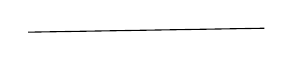
\begin{tikzpicture}\draw[line width=0.4pt] (0,0)--(3,0.05);\end{tikzpicture}}

De ces cogitations essentiellement géométriques, je ne saurais à l'heure actuelle tirer un programme précis de développement de structures algébriques adéquates pour les exprimer. Je me bornerai à quelques remarques en marge.

\deleted{\unsure{a|$\alpha$})} Depuis longtemps j'ai été \unsure{intrigu-|intrigué} par l'idée d'une ``linéarisation'' d'un type d'homotopie (ordinaire), i.e. la question du type: Si $X$ est un type d'homotopie, combien d'information cohomologique du type: cohomologie de $X$ à coefficients variables $M$ (constant%
% Detached compact point below the first constant, approximately (818,1807); origin uncertain.
\raisebox{0pt}[0pt][0pt]{\parbox{0pt}{\figure{\begin{tikzpicture}[overlay,x=1pt,y=1pt]\fill (-28,-7) circle[radius=0.35pt];\end{tikzpicture}}}} ou constant tordus),
% Detached short mark above the beginning of structure, approximately (272,1838); no textual value assigned.
\raisebox{0pt}[0pt][0pt]{\parbox{0pt}{\figure{\begin{tikzpicture}[overlay,x=1pt,y=1pt]\draw[line width=0.55pt] (8,15)--(8.4,13.5)--(8.7,13.6);\end{tikzpicture}}}}structure multiplicative $\deleted{\unsure{=|+}}H^i(X,M)\times H^j(X,N)\mathrel{\unsure{\dashv|\to|-}}H^{\unsure{i\cdot j|i+j|ij}}(X,M\otimes N)$, plus éventuellement d'autres opérations cohomologiques -- est-il%
% Detached angular stroke to the right of est-il, approximately (1619,2078); origin uncertain.
\raisebox{0pt}[0pt][0pt]{\parbox{0pt}{\figure{\begin{tikzpicture}[overlay,x=1pt,y=1pt]\draw[line width=0.55pt] (40,4)--(40.3,2.5)--(40.2,2)--(40.5,2.4)--(41.4,1.2);\end{tikzpicture}}}} nécessaire d'avoir pour réconstituer le type d'homotopie entièrement \deleted{\unsure{?}}? (disons,
